\documentclass[a4paper]{article}

\usepackage[french]{babel}
\usepackage[T1]{fontenc}
\usepackage[utf8]{inputenc}
\usepackage{amsmath}
\usepackage{graphicx}
\usepackage{lmodern}
\usepackage[left=3cm, right=3cm, bottom=4cm, top=4cm]{geometry}
\usepackage{array}
\usepackage{pdfpages}
\usepackage{rotating}
\usepackage[gen]{eurosym}
\DeclareUnicodeCharacter{20AC}{\euro{}}

\usepackage{hyperref}

\title{
\textsc{Jeu SmallWorld\\
\LARGE Rapport de conception}
}

\author
{
	Hyuk-Chan {\sc Kwon}\\
    Florent {\sc Mallard}\\
}

\date{\today}

\begin{document}
\maketitle
\begin{center}
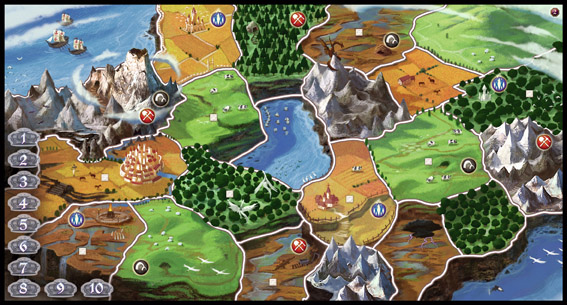
\includegraphics[width=0.8\textwidth]{./smallworld.jpg}~\\[5cm]
\end{center}

\newpage
\tableofcontents
\newpage


\section*{Introduction}
Le projet de Programmation et de Modélisation Orientée Objet se porte sur la réalisation d'un jeu inspiré de SmallWorld. Il s'agit d'un jeu de stratégie à deux joueurs dans lequel chacun dirige un peuple. Les unités des peuples bougent sur les cases de la carte afin de les conquérir, et combattent les unités ennemies. Le but est de contrôler plus de cases que son adversaire.\\
Nous allons aborder les thèmes principaux de la phase d'analyse et de conception.
Nous y expliquerons nos choix de conception  et de modélisation de notre jeu. Nous commencerons par effectuer un rappel des règles afin de distinguer les actions possibles.
Les étapes d'analyse ainsi que les différents diagrammes (classe, séquence, cas d'utilisation) figurent également dans ce rapport.
Nous expliquerons également notre utilisation des patrons de conception.

\section{Principes et But du jeu}
	\subsection{Règles du jeu}
		\subsubsection{Peuples}
Les joueurs ont le choix entre trois peuples : les Orcs, les Elfs et les Nains. Chacun dispose de bonus et malus influant sur la façon de les jouer.

\paragraph{Elfs} Les Elfs ont un coût de déplacement réduit de moitié sur une case Forêt, tandis que le déplacement sur une case Déserte est deux fois plus coûteux. Lors d'un combat dont l'issue conduit à la mort de l'unité, celle-ci a 50\% de chance de s'échapper avec 1 point de vie.
\paragraph{Orcs} Les Orcs ont un coût de déplacement 50\% sur une case Plaine. Ils ne gagnent aucun point sur une case Forêt, mais ont un bonus propre à l'unité lorsque celle-ci en tue une autre.
\paragraph{Nains} Les Nains ont un coût de déplacement divisé par deux sur une case Plaine. Ils n'acquièrent aucun point sur les cases de ce type. Ils peuvent se déplacer d'une case Montagne à une autre à condition que celle-ci ne soit pas occupée par une unité adverse.

		\subsubsection{Cartes}
Le joueur, à la création de la partie, a le choix entre trois cartes :
\begin{itemize}
\item Démo : 2 joueurs, 5 cases x 5 cases, 5 tours, 4 unités par peuple.
\item Petite : 2 joueurs, 10 cases x 10 cases, 20 tours, 6 unités par peuple.
\item Normale : 2 joueurs, 15 cases x 15 cases, 30 tours, 8 unités par peuple.
\end{itemize}

		\subsubsection{Déroulement d'une partie}
Au début du jeu, chaque joueur choisit son peuple. Chaque peuple débute la partie avec toutes ses unités sur la même case de la carte, choisie de manière à ce que les joueurs ne soient pas trop proches. L’ordre de jeu est déterminé aléatoirement en début de partie. Les joueurs jouent chacun leur tour sur le même ordinateur.

	\subsection{Tours de jeu}
Lorsqu’un joueur peut jouer (c.-à-d. une fois par tour), il peut déplacer toutes ses unités suivant leur nombre de points de déplacements (un déplacement sur une case coûte un point de déplacement). Il est possible pour chaque unité de passer son tour (généralement par le biais de la touche espace). Une unité combattante peut engager un combat s’il lui reste au moins un point de mouvement. Lorsqu’un joueur a fini son tour, il clique sur le bouton correspondant ("Fin tour"). C’est alors au joueur suivant de commencer son tour. La partie se termine lorsque le nombre de tours prédéfini en début de partie à été effectué, ou lorsqu’il ne reste qu’un seul joueur sur le plateau.

\section{Analyse}
	
Après avoir lancé le jeu, l'utilisateur a la possibilité de créer une nouvelle partie, ou bien d'en charger une existante.
	
	\subsection{Lancement d'une partie}
La Figure \ref{fig:cas_creation} représente la création d'une partie. Le joueur A choisit son nom de joueur puis son peuple. Le joueur B fait de même, puis définit la taille de la carte. Celui-ci termine en lançant la partie. Nous avons donc défini la machine à état globale du jeu, et le diagramme de séquence associé, respectivement en Figure \ref{fig:machine_jeu} et en Figure \ref{fig:sequence_creation}

\begin{figure}[ht]
\centering
	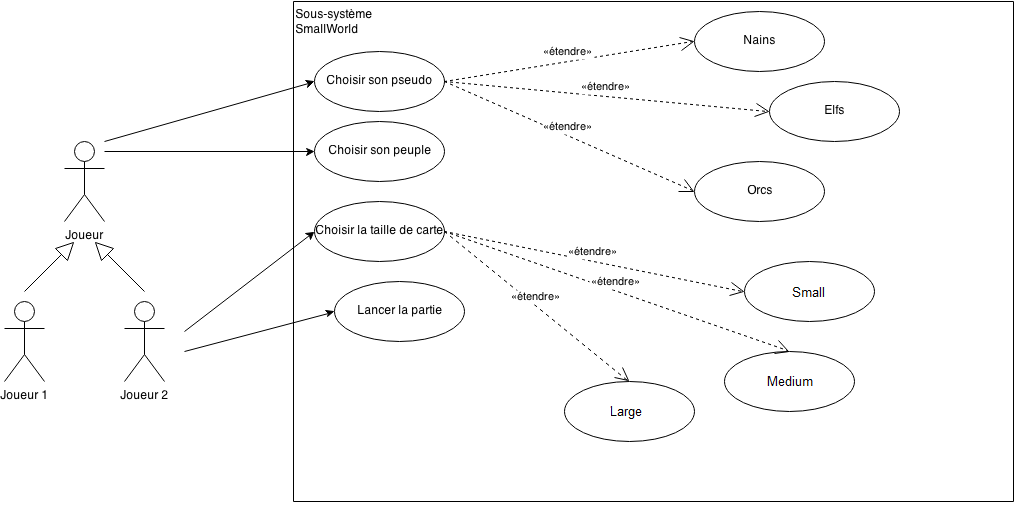
\includegraphics[width=1\textwidth]{../Schemas/CU_Creation.png}
		\caption{Diagramme de cas d'utilisation de création du jeu}
		\label{fig:cas_creation}
\end{figure}

\begin{figure}[ht]
\centering
	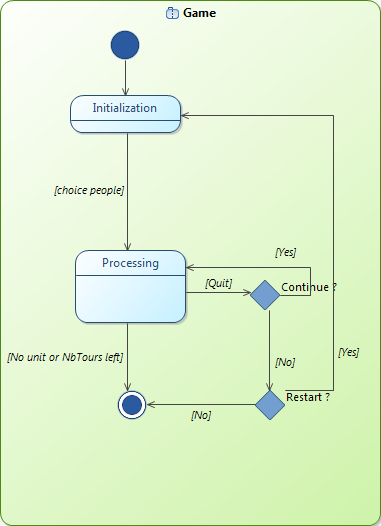
\includegraphics[width=0.65\textwidth, height=0.5\textheight]{../Schemas/machine_etat_jeu.png}
		\caption{États globaux du jeu}
		\label{fig:machine_jeu}
\end{figure}

\begin{figure}[ht]
\centering
	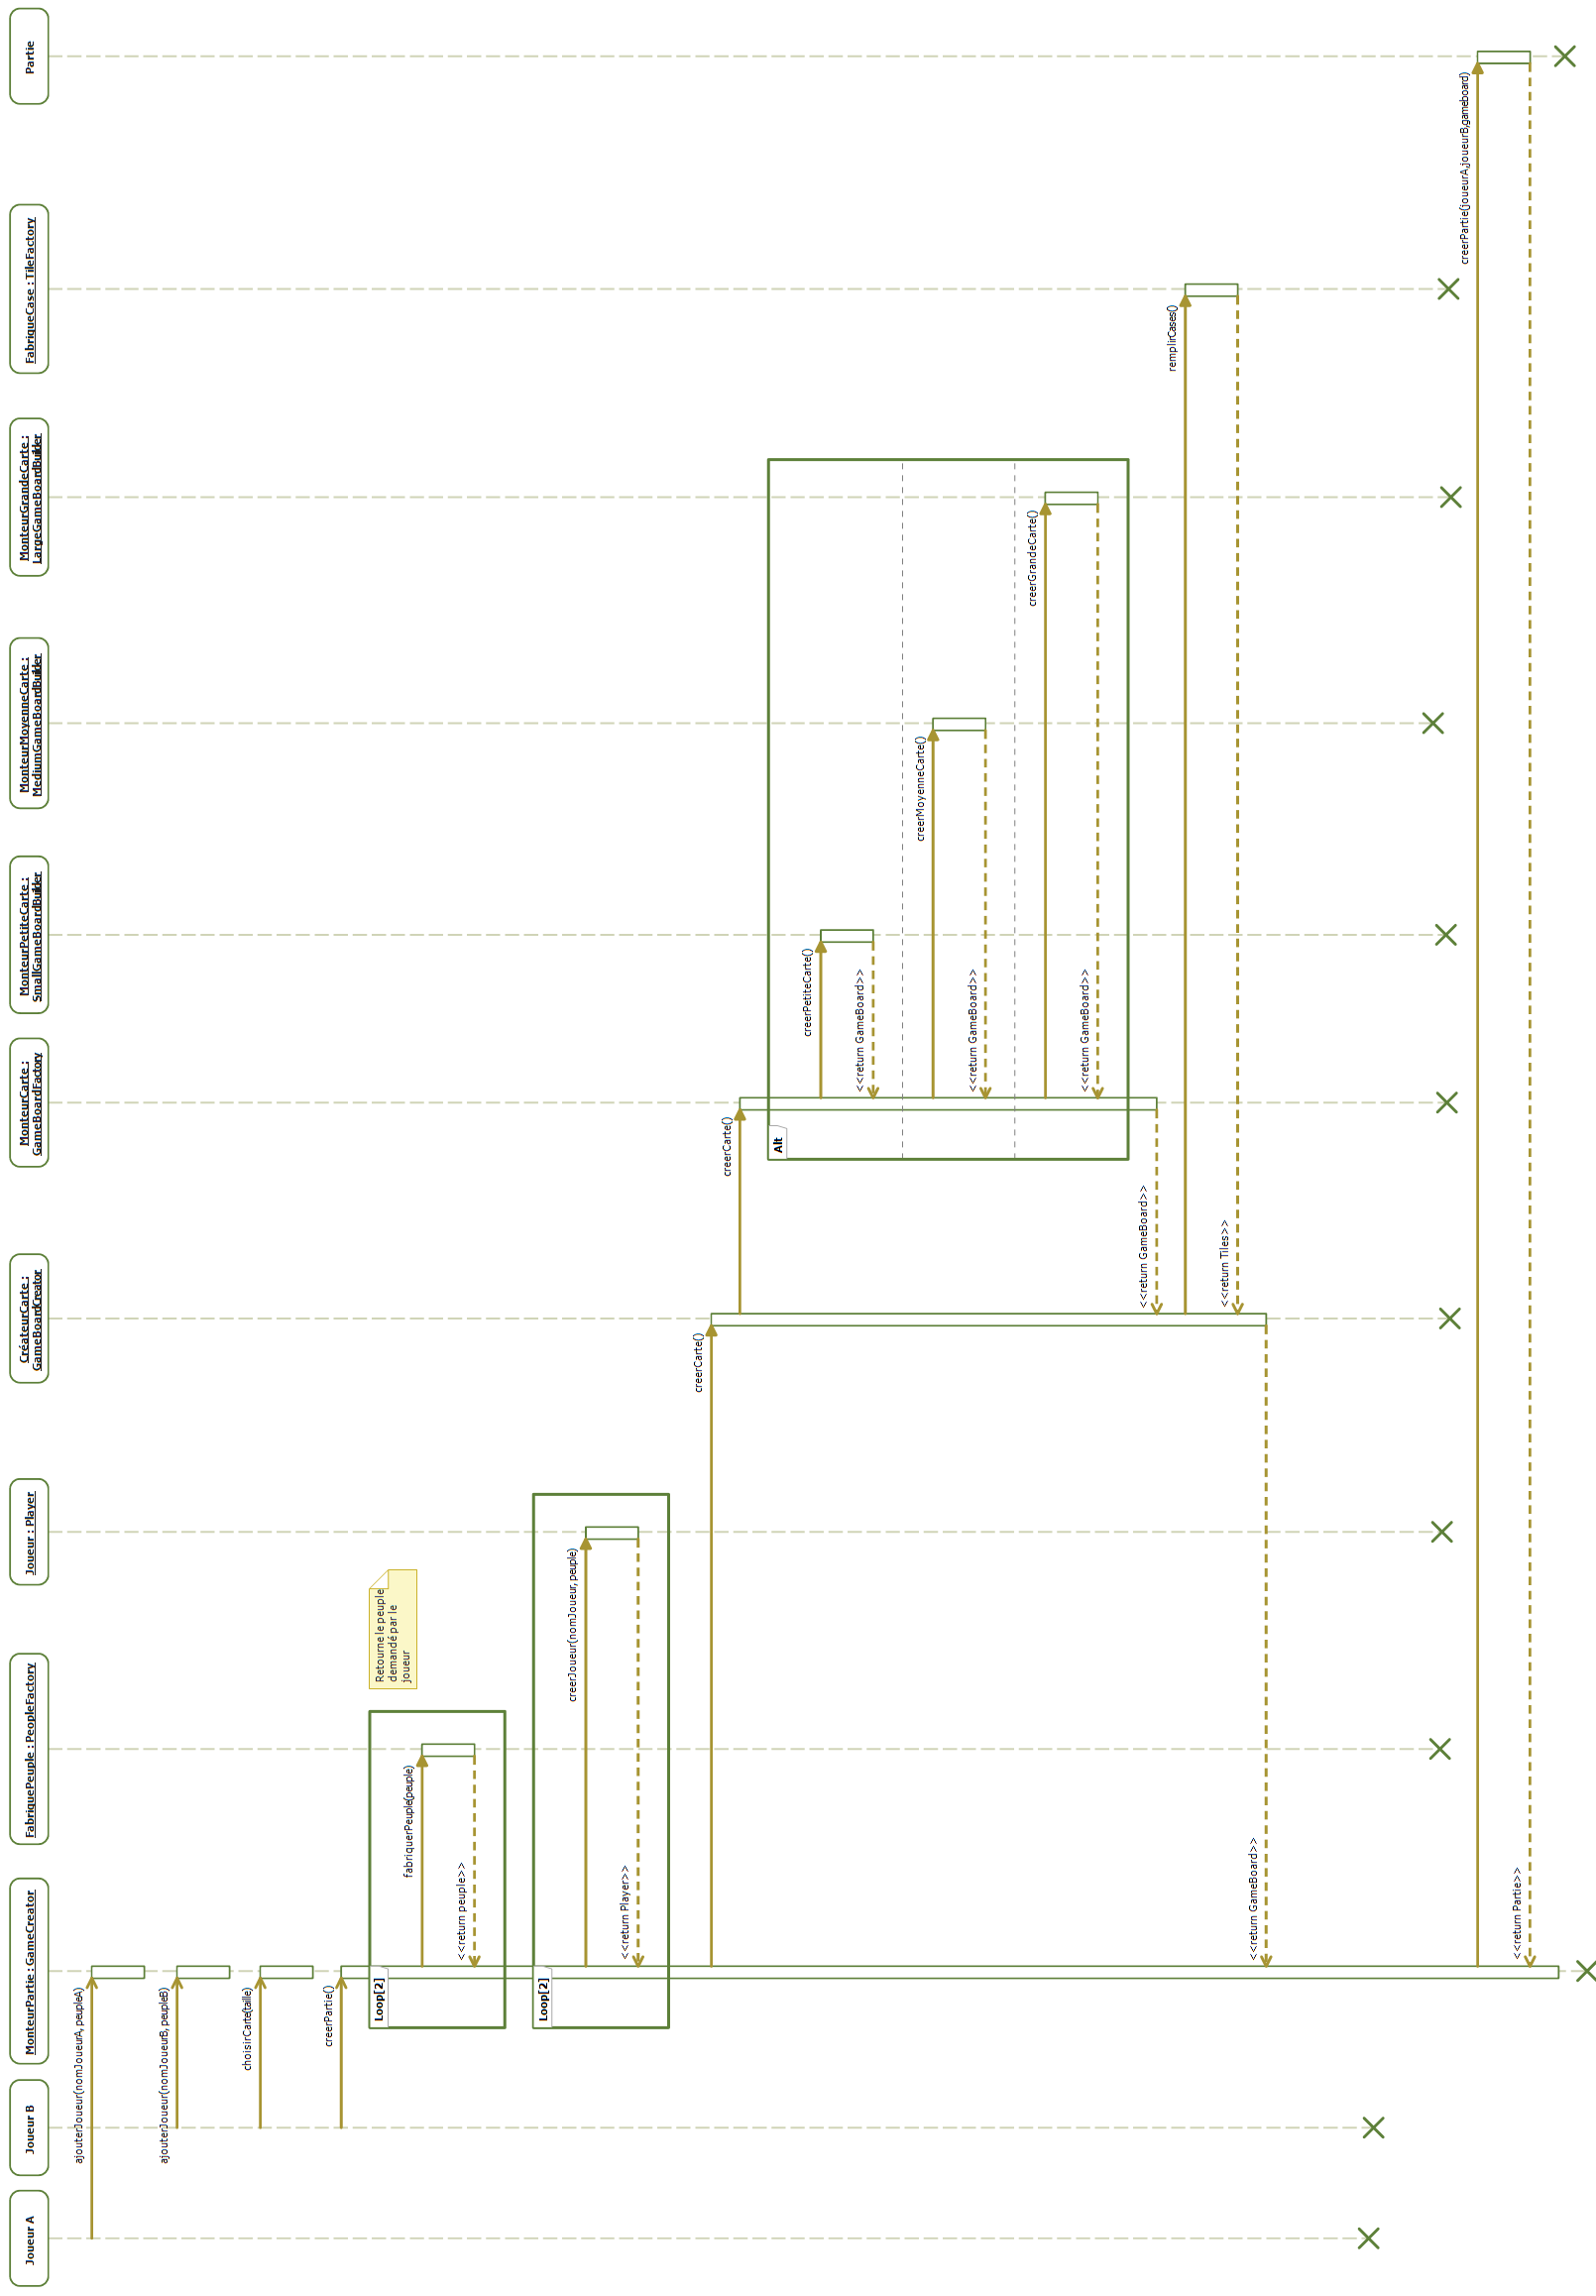
\includegraphics[width=0.9\textwidth, height=0.9\textheight]{../Schemas/sequence_creerPartie.png}
		\caption{Séquences pour la création du jeu}
		\label{fig:sequence_creation}
\end{figure}

\clearpage
	\subsection{Tour de jeu}
Nous avons représenté un tour de jeu avec la Figure~\ref{fig:cas_tour}. Le joueur peut déplacer chaque unité selon son nombre de points de déplacement, et le coût de celui-ci (par défaut bouger d'une case coûte un point). En cas de rencontre d'une unité adverse, un combat a lieu. Il peut également passer le tour de l'unité, ou terminer totalement son tour. L'annulation d'un déplacement est prévue, ainsi que la sauvegarde de la partie. Le déroulement de ces actions est représenté sur la Figure \ref{fig:inter_tour}

\begin{figure}[ht]
\centering
	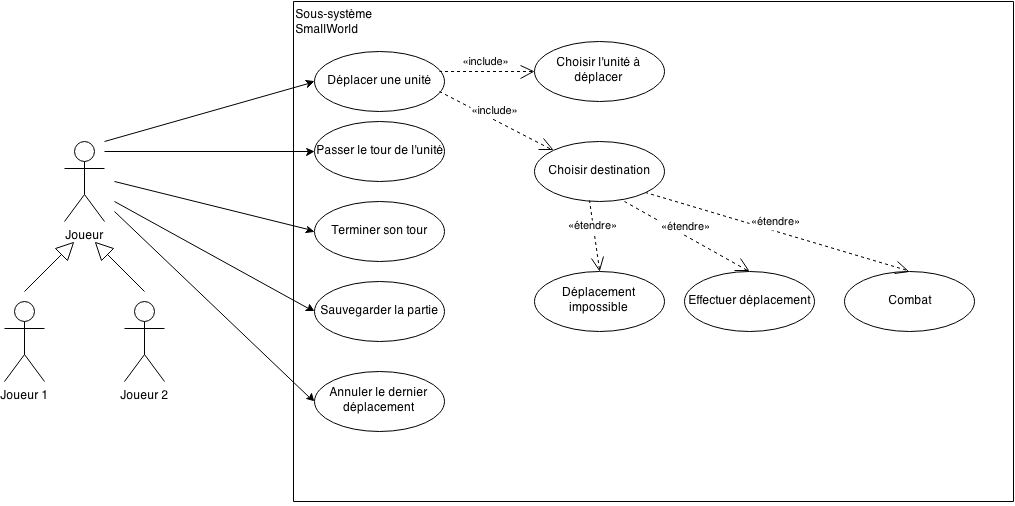
\includegraphics[width=1\textwidth]{../Schemas/CU_Tour.png}
		\caption{Diagramme de cas d'utilisation d'un tour de jeu}
		\label{fig:cas_tour}
\end{figure}

\begin{figure}[ht]
\centering
	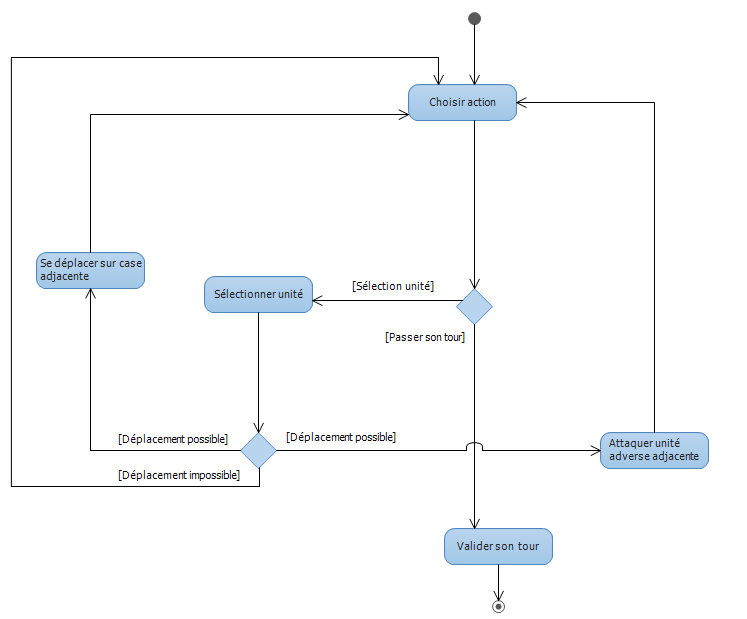
\includegraphics[width=1\textwidth]{../Schemas/Interaction_Tour.png}
		\caption{Diagramme d'interaction d'un tour de jeu}
		\label{fig:inter_tour}
\end{figure}
\clearpage
	\subsection{Combat}
 A la rencontre d'unités adverses, le joueur peut décider de combattre à l'aide de ses unités. Le déroulement d'un combat est montré à l'aide de la Figure~\ref{fig:interaction_combat}.
\begin{figure}[ht]
\centering
	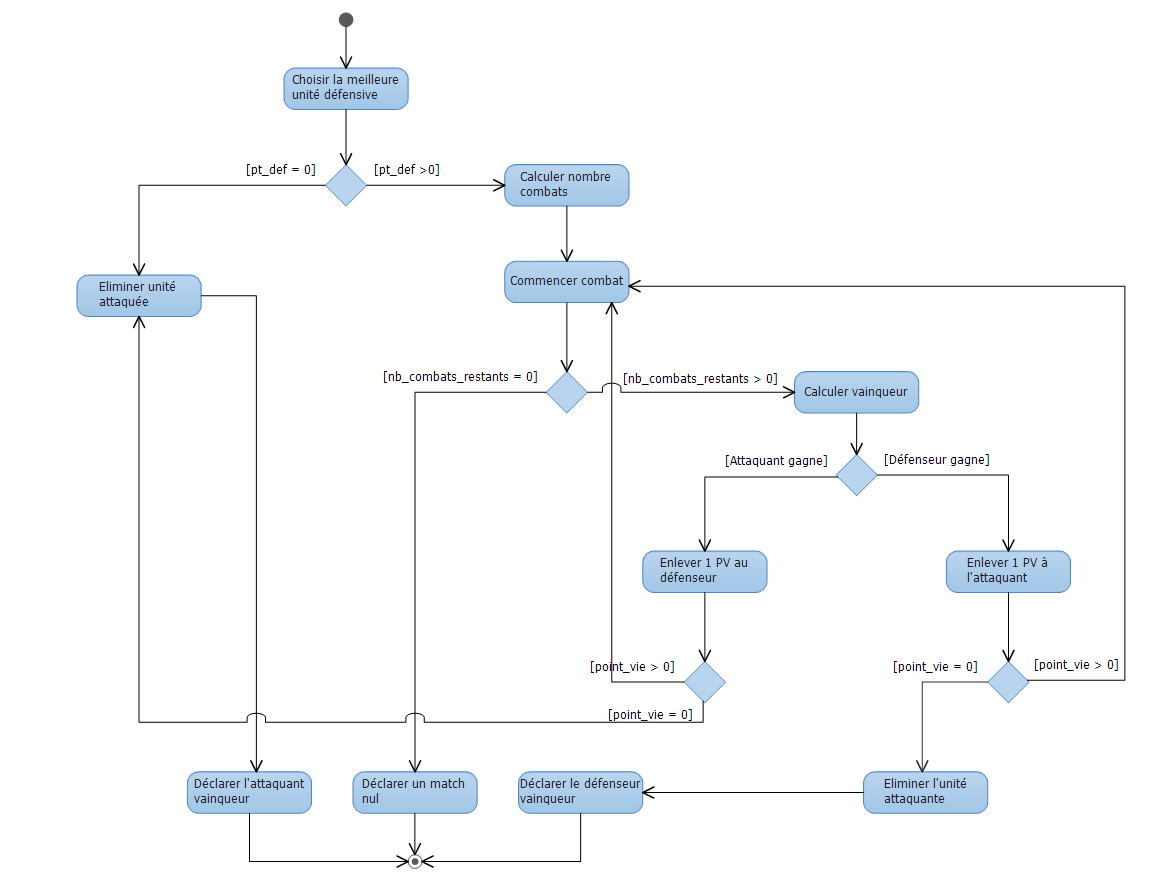
\includegraphics[width=1\textwidth, height=0.4\textheight]{../Schemas/Interaction_Combat.png}
		\caption{Diagramme d'interaction représentant un combat}
		\label{fig:interaction_combat}
\end{figure}

Les calculs des combats prennent en compte les points de vie restants de chaque unité en combat, pour déterminer des probabilités de remporter le combat. Une attaque est composée de 3 au maximum des points de vie des unités en combat + 2. Chaque combat fait perdre un point de vie à l'unité perdante, jusqu'à ce que le nombre de combats soit atteint ou qu'une unité soit tuée.

\clearpage
	\subsection{Unités}
Le diagramme d'état-transitions, Figure\ref{fig:machine_unite}, montre le cycle de vie d'une unité. Une unité peut simplement être vivante ou non.
A sa création, elle possède cinq points de vie.
Au début d'un tour, l'unité possède un point de déplacement. Elle a alors la possibilité de se déplacer. Si elle rencontre une unité ennemie, elle combat et en ressort soit vainqueure (ou match nul), soit perdante. Dans ce dernier cas l'unité meurt et atteint son état final.

\begin{figure}[ht]
\centering
	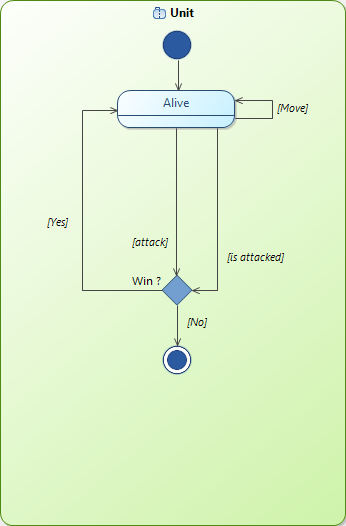
\includegraphics[width=0.5\textwidth, height=0.4\textheight]{../Schemas/machine_etat_unite.png}
		\caption{Machine à état pour une unité}
		\label{fig:machine_unite}
\end{figure}

\clearpage
\section{Modélisation et diagrammes de classe}
Nous allons dans cette section expliquer nos utilisations des différents patrons de conception, accompagnés de diagrammes de classe montrant leur mise en place au sein de notre de conception.
	
	\subsection{Fabrique}
Le patron de conception \textit{Fabrique} est utilisé pour la création des différents peuples. En effet, le jeu créera simplement un peuple, sans savoir duquel il s'agit. Une interface réunit les points commun entre les différents peuples. Les unités étant toutes les mêmes, elles n'ont pas besoin de \textit{Fabrique}. Les classes sont représentées dans la Figure \ref{fig:class_factory}

\begin{figure}[ht]
\centering
	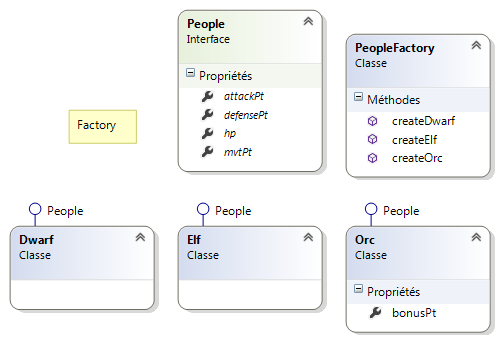
\includegraphics[width=\textwidth]{../Schemas/class_People_Factory.png}
		\caption{Fabrique des différents peuples}
		\label{fig:class_factory}
\end{figure}

\clearpage
	\subsection{Monteur}
Nous avons utilisé un \textit{Monteur} pour la création d'une partie. En effet, la création d'une partie est un assemblage de différents objets complexes. Son utilisation extériorise la création d'une partie, et permettra de pouvoir implémenter les différentes configurations de partie. Il est représenté à la Figure~\ref{fig:class_builder}.

\begin{figure}[ht]
\centering
	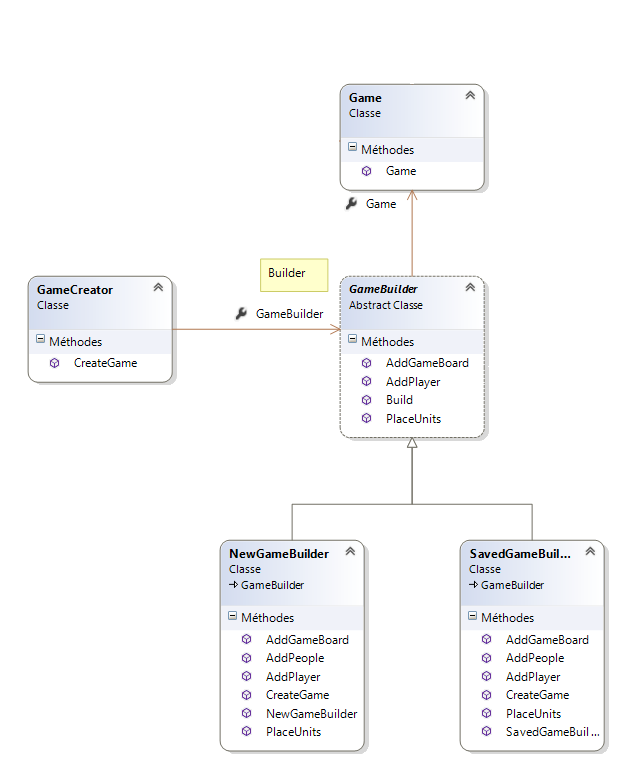
\includegraphics[width=\textwidth]{../Schemas/class_GameBoardBuilder_Builder.png}
		\caption{Monteur de la partie}
		\label{fig:class_builder}
\end{figure}

\clearpage
	\subsection{Stratégie}
Le patron de conception \textit{Stratégie} est utilisé pour la création des cartes. En effet, le joueur a la choix entre trois tailles : Petite, Moyenne et Grande. Cette implémentation nous permettra de changer facilement d'algorithmes en fonction de ce choix, et d'en implémenter de nouveaux au besoin. Cette modélisation est représentée à la Figure \ref{fig:class_strategy}.

\begin{figure}[ht]
\centering
	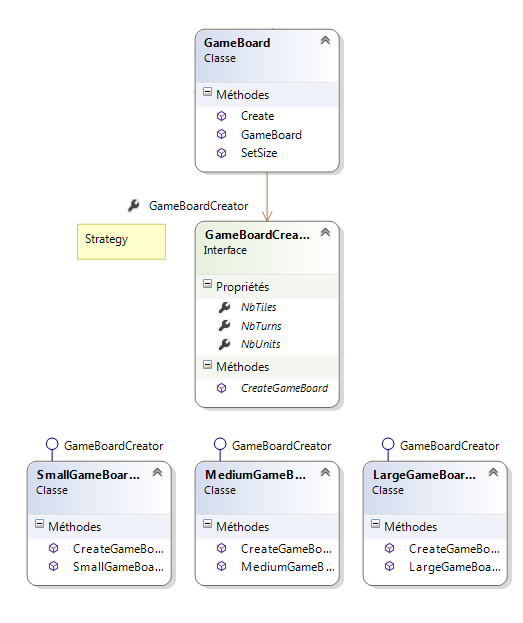
\includegraphics[width=\textwidth]{../Schemas/class_GameBoardBuilder_Strategy.png}
		\caption{Stratégie de création de la carte}
		\label{fig:class_strategy}
\end{figure}

\clearpage
	\subsection{Poids-mouche}
La carte est composée de cases de quatre types : Montagne, Plaine, Désert et Forêt. Instancier chaque case consommerait beaucoup de mémoire, c'est pourquoi nous utilisons le \textit{Poids-Mouche}. Ce modèle permet de ne pas créer plusieurs fois le même type de case. La Figure \ref{fig:class_poidsmouche} illustre ce patron. Nous utilisons également une \textit{Fabrique} pour la création aléatoire des cases de la carte.

\begin{figure}[ht]
\centering
	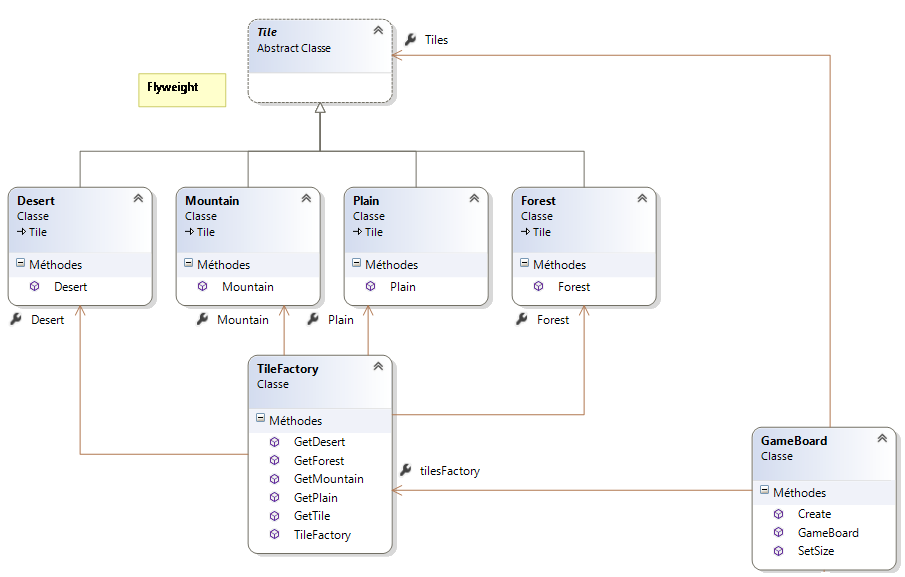
\includegraphics[width=\textwidth]{../Schemas/class_GameBoard_PoidsMouche.png}
		\caption{Poids-Mouche pour les cases de la carte}
		\label{fig:class_poidsmouche}
\end{figure}

\clearpage
	\subsection{Diagramme de classes global}
Voici donc la représentation globale de notre projet, visible à la Figure \ref{fig:class_global}.

\begin{figure}[ht]
\centering
	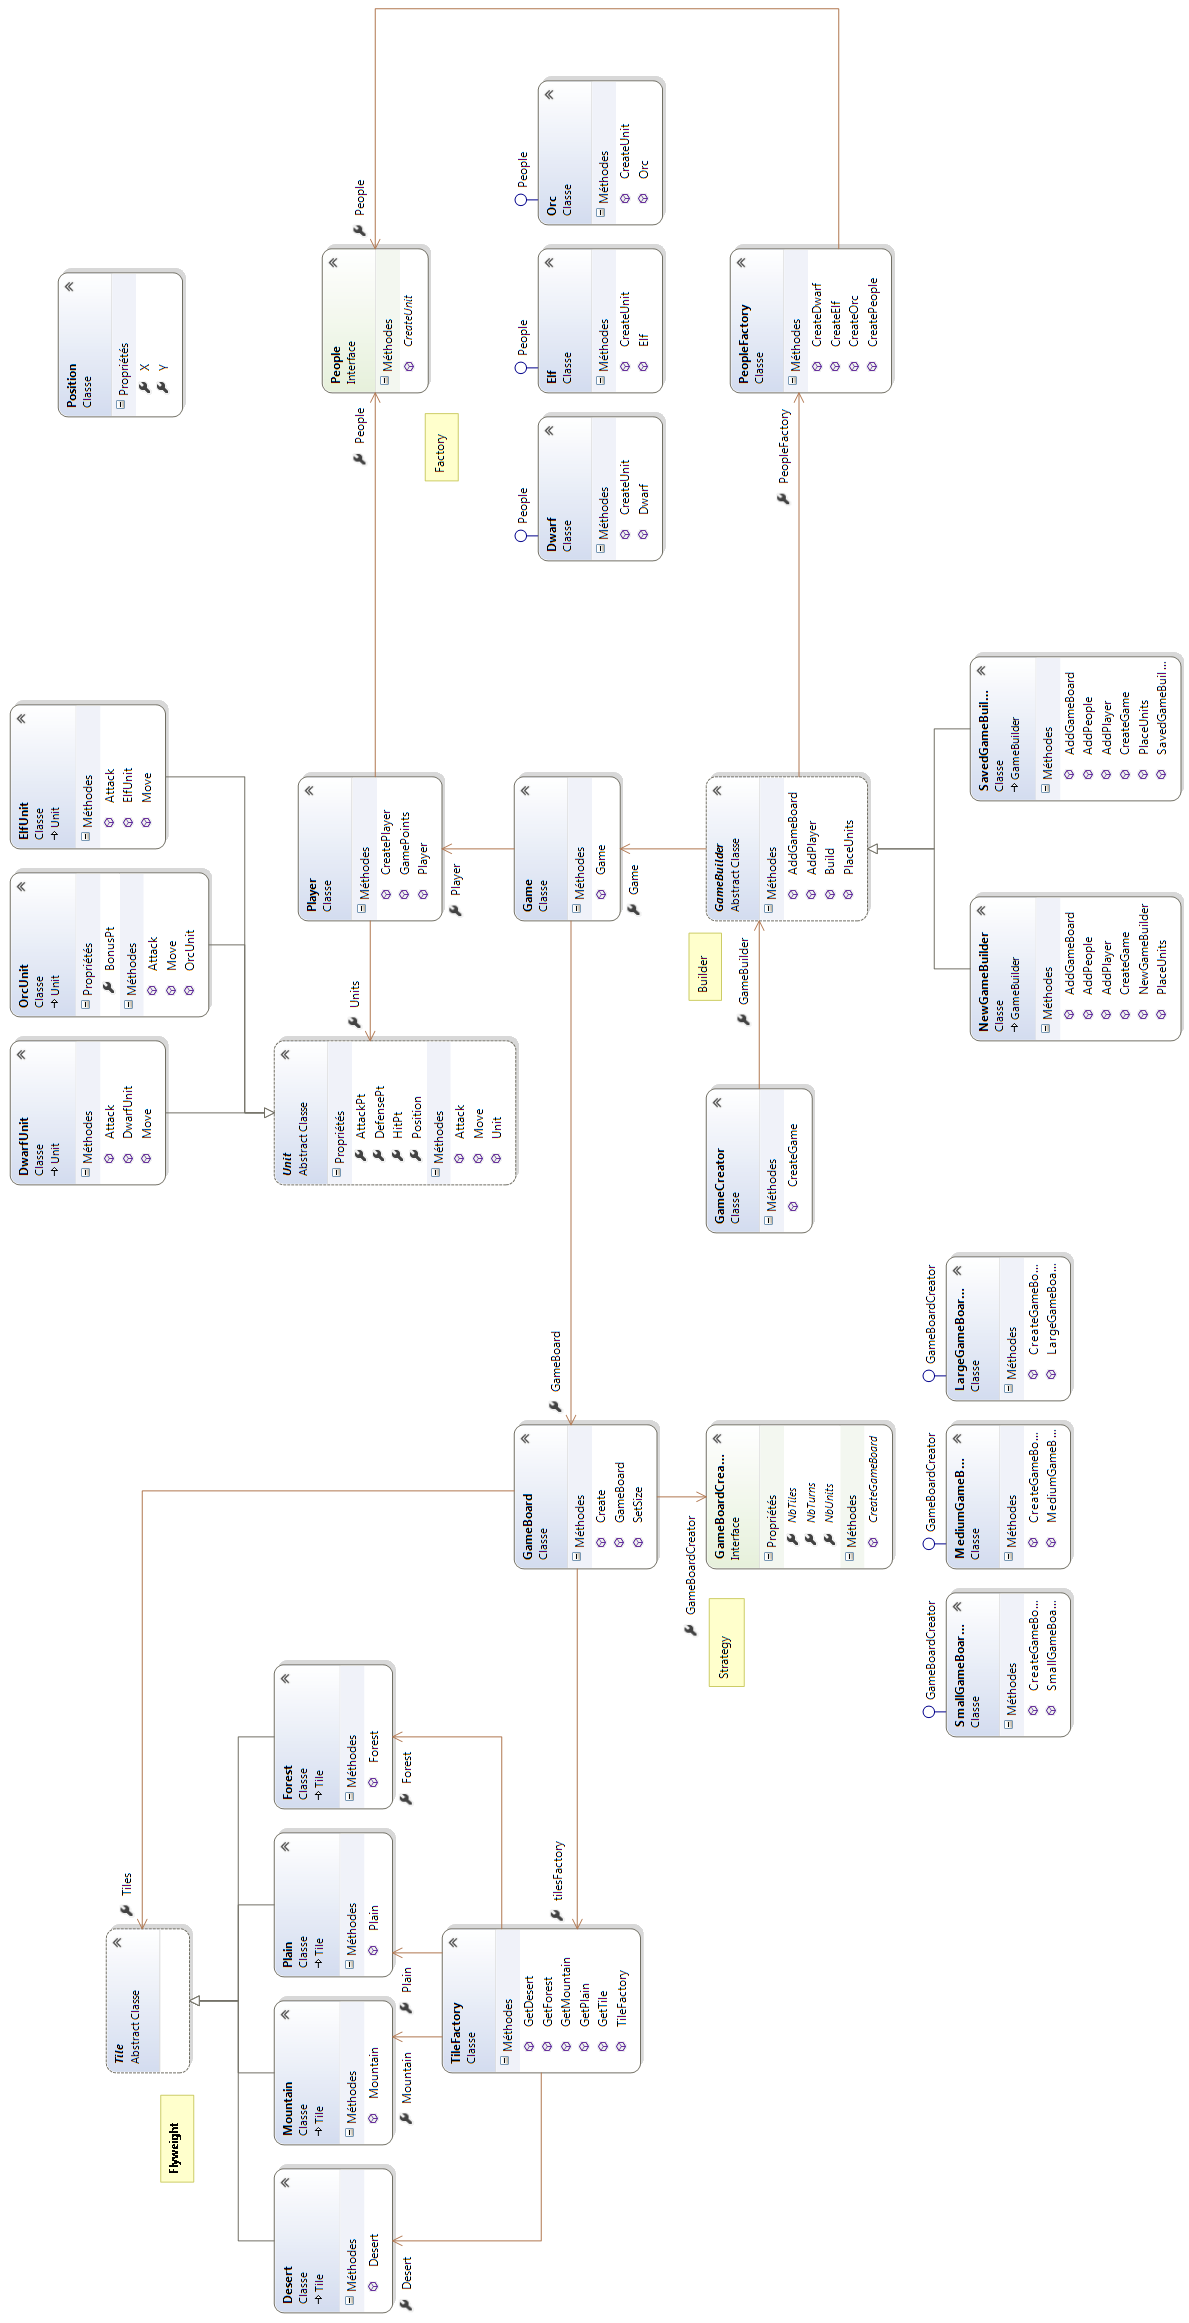
\includegraphics[width=0.8\textwidth, height=0.74\textheight]{../Schemas/class_global.png}
		\caption{Diagramme de classes complet}
		\label{fig:class_global}
\end{figure}

\clearpage
\section{Conclusion}
\newpage
\listoffigures
\end{document}